\section{Experiments}
\label{sec:intro}

We conducted three different experiments where we evaluated the accuracy of the models in terms of how many test commands were exactly translated
into corresponding test actions. Unless otherwise stated, average across 5 different runs and standard deviation are reported.
\citet{Lake:Baroni:2017} found that RNNs models are achieve nearly perfect performance when tested on a random split of SCAN but accuracy drops significantly
(down to around 20\% for their best performing model) when the network is tested on composing new meanings after being exposed only to shorter samples.

In order to make our results comparable with previous work on SCAN each training set consists of 100K examples sampled with replacement
from each related train/test split. We decided to replicate experiment 1 of \cite{Lake:Baroni:2017} that simply uses a random split
of the SCAN dataset divided into a train (80\%) and test (20\%) set. This would act as a first comparison with the RNNs results reported in their work.

\subsection{Experiment 1: random split and primitive generalization}
\label{subsec:exp1}

\begin{figure}[h]
    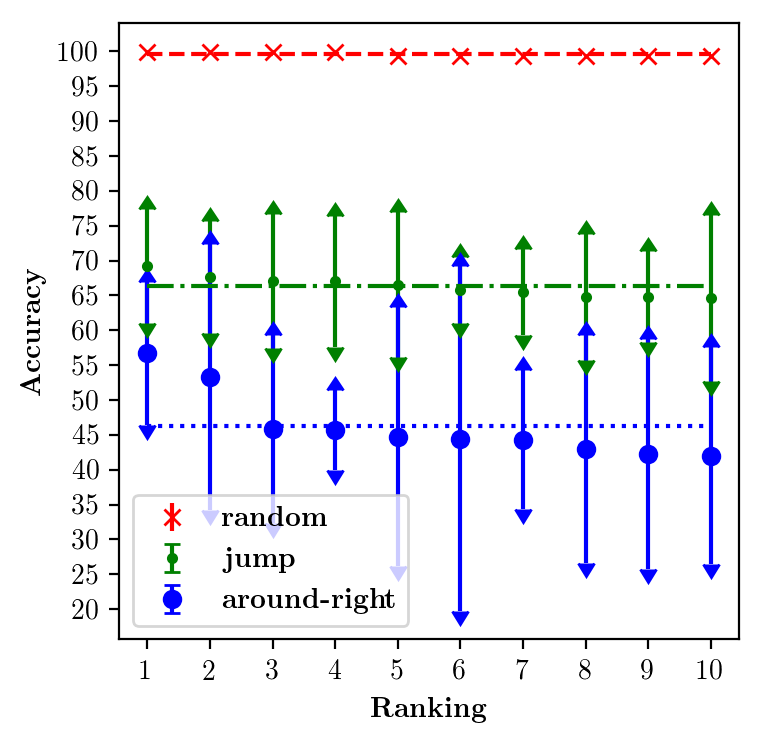
\includegraphics[width=.5\textwidth,keepaspectratio]{figures/accuracies_all_splits.png}
    \centering
    \caption{All splits accuracies}
    \label{fig:accuracy_all_splits}
\end{figure}

% 219.08612pt
% 3.0314
\subsection{Experiment 2: second-order modifiers and kernel study}
\label{subsec:exp2}

\begin{figure}[h]
    \centering
    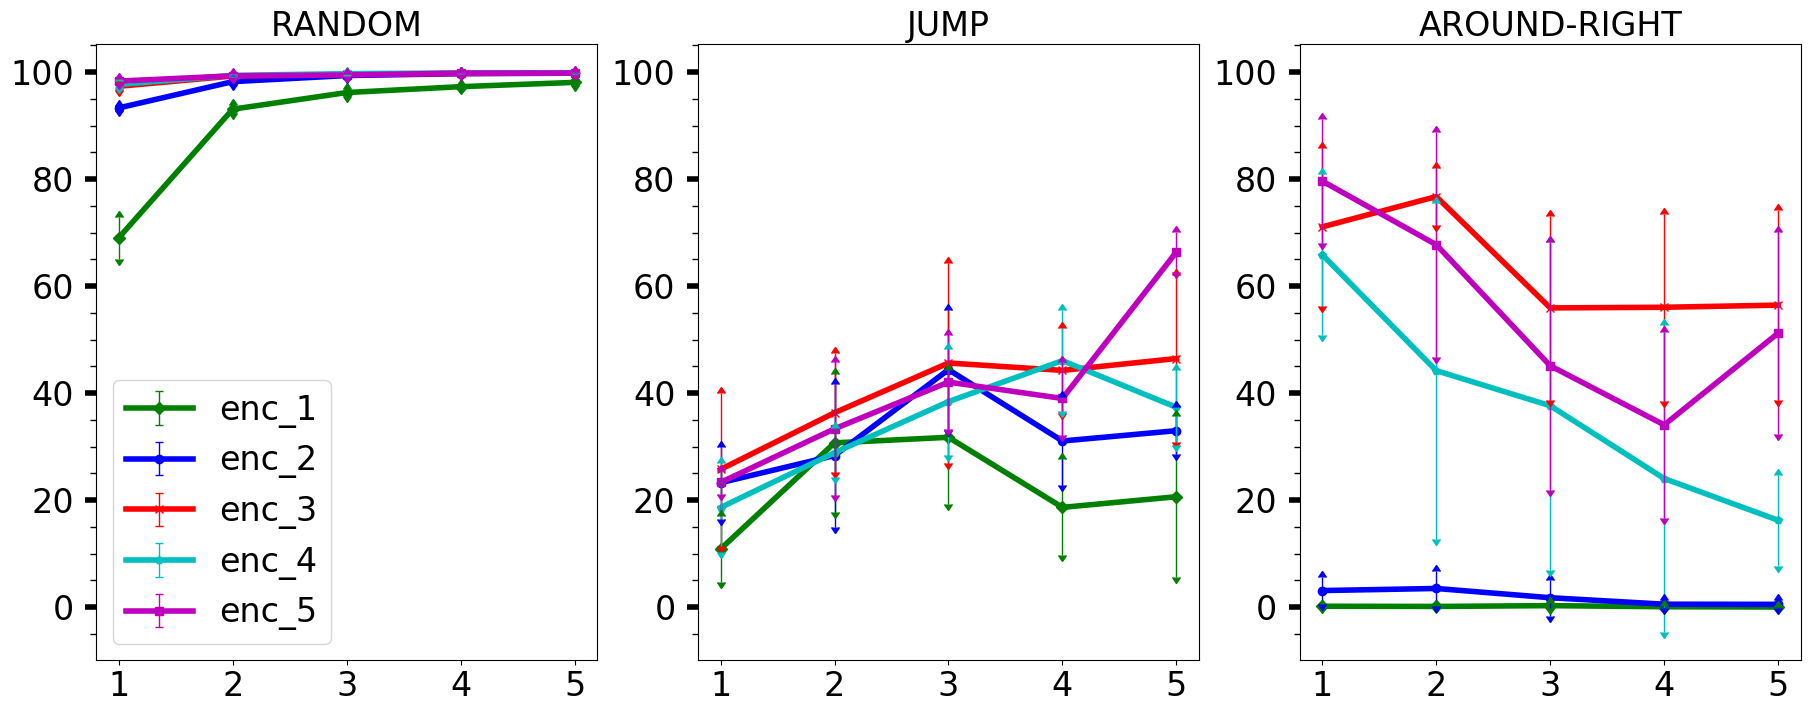
\includegraphics[width=80mm, height=150mm,keepaspectratio]{figures/kernel_exp.png}
    \caption{Accuracy for kernel experiment}
    \label{fig:kernel_exp}
\end{figure}

\subsection{Experiment 3: ablation study on attention}
\label{subsec:exp3}

\begin{figure}[h]
    \centering
    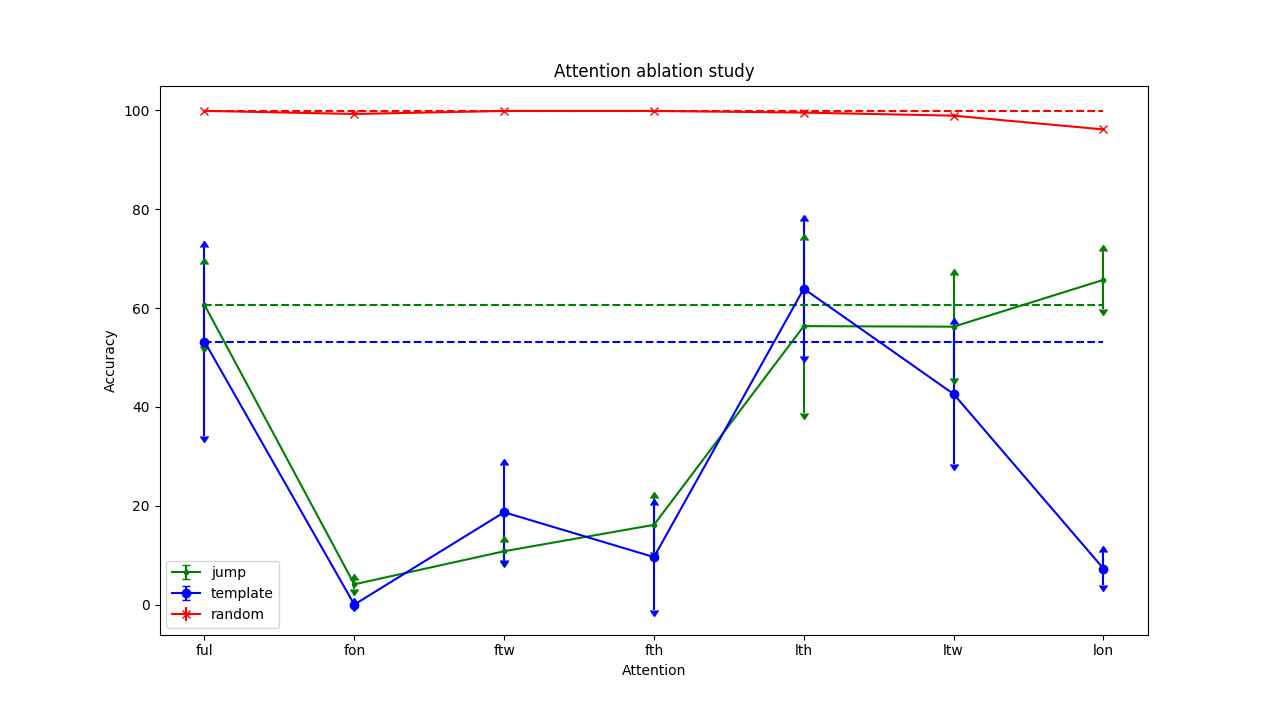
\includegraphics[width=80mm, height=150mm,keepaspectratio]{figures/attention_exp.png}
    \caption{Accuracy for attention experiment}
    \label{fig:attention_exp}
\end{figure}


